\documentclass{article}
\usepackage[utf8]{inputenc}
\usepackage[T1]{fontenc}
\usepackage[brazil]{babel}
\usepackage{geometry}
\usepackage{graphicx}
\usepackage{float}
\usepackage{array}
\usepackage{booktabs}
\usepackage{amsmath}
\usepackage{hyperref}

\title{Roteiro 1}
\author{Ana Beatriz Barbosa Yoshida - RA: 245609 \\ Julio Nunes Avelar - RA: 241163}
\date{Agosto de 2025}

\begin{document}

\maketitle

\tableofcontents
\newpage

% ---------------- Experiência 1 ----------------
\section{Experiência 1}

\subsection{1.1 Identificação das GPIOs do LED RGB}
\begin{itemize}
    \item Vermelho: GPIO 13 com resistor de 220 $\Omega$
    \item Verde: GPIO 11 com resistor de 220 $\Omega$
    \item Azul: GPIO 12 com resistor de 150 $\Omega$
\end{itemize}

\subsection{1.2 Níveis lógicos do RP2040}
\begin{itemize}
    \item Nível lógico 0: 0 V
    \item Nível lógico 1: 3.3 V
\end{itemize}

\subsection{1.3 Circuito básico e cálculo dos resistores}
Inserir desenho esquemático do circuito do LED RGB.  
\begin{figure}[H]
    \centering
    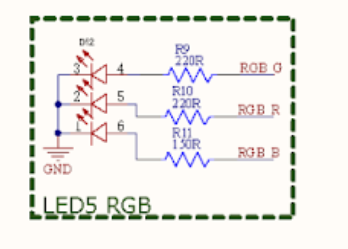
\includegraphics[width=0.6\textwidth]{circuito_led.png}
    \caption{Circuito do LED RGB com resistores.}
\end{figure}

Cálculo do resistor (Lei de Ohm):  
\[
R = \frac{V_{CC} - V_{LED}}{I_{LED}}
\]

% -------- Tarefa 1.1 --------
\subsection{Tarefa 1.1 -- Comparação entre linguagens}
Sugestão de método: medir tempo de execução de funções idênticas em C e MicroPython utilizando cronômetro interno.  

\begin{table}[H]
    \centering
    \begin{tabular}{lcc}
        \toprule
        Linguagem & Tempo de Resposta (ms) & Observações \\
        \midrule
        C          & ... & ... \\
        MicroPython & ... & ... \\
        \bottomrule
    \end{tabular}
    \caption{Benchmark básico entre C e MicroPython.}
\end{table}

% -------- Tarefa 1.2 --------
\subsection{Tarefa 1.2 -- Comparativo Imperativo vs OO}
\begin{table}[H]
    \centering
    \begin{tabular}{lcccc}
        \toprule
        Paradigma & Linguagem & Tamanho Código (bytes) & Tempo de Resposta (ms) & Observações \\
        \midrule
        Imperativo & C & ... & ... & ... \\
        OO & C & ... & ... & ... \\
        Imperativo & Python & ... & ... & ... \\
        OO & Python & ... & ... & ... \\
        \bottomrule
    \end{tabular}
    \caption{Benchmark entre Imperativo e OO em C e Python.}
\end{table}

% ---------------- Experiência 2 ----------------
\section{Experiência 2}

\subsection{2.1 GPIOs conectados aos botões}
Listar aqui cada botão e a respectiva GPIO.  

\subsection{2.2 Limites de tensão para nível lógico}
\begin{itemize}
    \item Nível baixo: $V < V_{IL(max)}$
    \item Nível alto: $V > V_{IH(min)}$
\end{itemize}

\subsection{2.3 Esquema dos botões}
\begin{figure}[H]
    \centering
    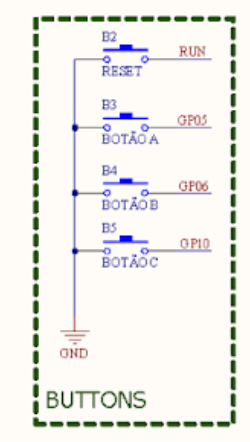
\includegraphics[width=0.6\textwidth]{circuito_botoes.png}
    \caption{Conexão dos botões ao RP2040.}
\end{figure}

\subsection{Debounce, Polling e IRQ}
\paragraph{Funcionalidade:} Confirmar alternância do LED nos dois modos.  
\paragraph{Latência:} Descrever efeito do aumento da carga em Polling e comparação com IRQ.  
\paragraph{Consumo de energia:} Justificar eficiência do IRQ.  
\paragraph{Aplicações:} Exemplos reais para Polling e IRQ.  

\subsection{Tabela Comparativa -- Polling × IRQ}
\begin{table}[H]
    \centering
    \begin{tabular}{lcc}
        \toprule
        Critério & Polling & IRQ \\
        \midrule
        Latência percebida & ... & ... \\
        Perdas de eventos & ... & ... \\
        Consumo de CPU & ... & ... \\
        Complexidade & ... & ... \\
        Situações suficientes & ... & ... \\
        Situações obrigatórias & ... & ... \\
        \bottomrule
    \end{tabular}
    \caption{Comparativo Polling vs IRQ.}
\end{table}

% ---------------- Experiência 3 ----------------
\section{Experiência 3}

\subsection{Demonstração}
Vídeo no YouTube: \url{https://youtube.com/xxxxxx} \#EA701  

\subsection{Comparação de código}
Comparar simplicidade entre Python OO e C modular.  

\subsection{Reflexão: IRQ + OO}
Discutir casos vantajosos em sistemas embarcados reais.  

\subsection{Expansão para 10 botões}
Discutir viabilidade de Polling vs IRQ.  

% ---------------- Conclusão ----------------
\section{Conclusão}
Resumo dos resultados, aprendizados e recomendações para projetos futuros.  


\end{document}
